\title{Ground survey to assess hemlock sawfly population during a large-scale outbreak in Southeast Alaska}

\subtitle{\doi{10.----------}}

\author{by Elizabeth Graham\footnote{USDA Forest Service R10, Forest Health Protection}}

\maketitle

\section{Introduction}

Hemlock sawfly (Hymenoptera: Diprionidae \textit{Neodiprion tsugae}, Figure \ref{hemlock_sawfly_larvae}) is an important defoliator of hemlock (\textit{Tsuga} spp.)  throughout its range from the panhandle of Southeast Alaska through coastal British Columbia, Washington and Oregon as well as in Interior British Columbia, Idaho and Montana \citep{Hardetal1976}.  Significant outbreaks have been recorded during aerial detection surveys in Southeast Alaska since the mid-1960’s (Figure Hemlock Sawfly damage graph) and there were reports of a major outbreak impacting all of the Tongass National Forest during the mid-1950’s. Western hemlock (\textit{Tsuga heterophylla}) is the preferred host, however they also feed on mountain hemlock (\textit{Tsuga mertensiana}) as well as Sitka spruce (\textit{Piceae sitchensis}) and occasionally other conifers.  The larvae feed on the older needles, avoiding the new growth, often only eating half of the needle, a feeding pattern called “wasterful feeding” (Figure Wasteful Feeder).  Because the important new foliage is retained feeding damage from hemlock sawfly rarely result in mortality, though it can result in topkill and reduction in radial growth.  Mortality can occur when outbreaks of hemlock sawfly coincide with a western blackheaded budworm outbreak (\textit{Acleris gloverana} (Figure western blackheaded budworm larvae)), which feed in the buds and new foliage resulting in complete defoliation. 

\begin{figure}[H]
\begin{center}
\vspace{2mm}
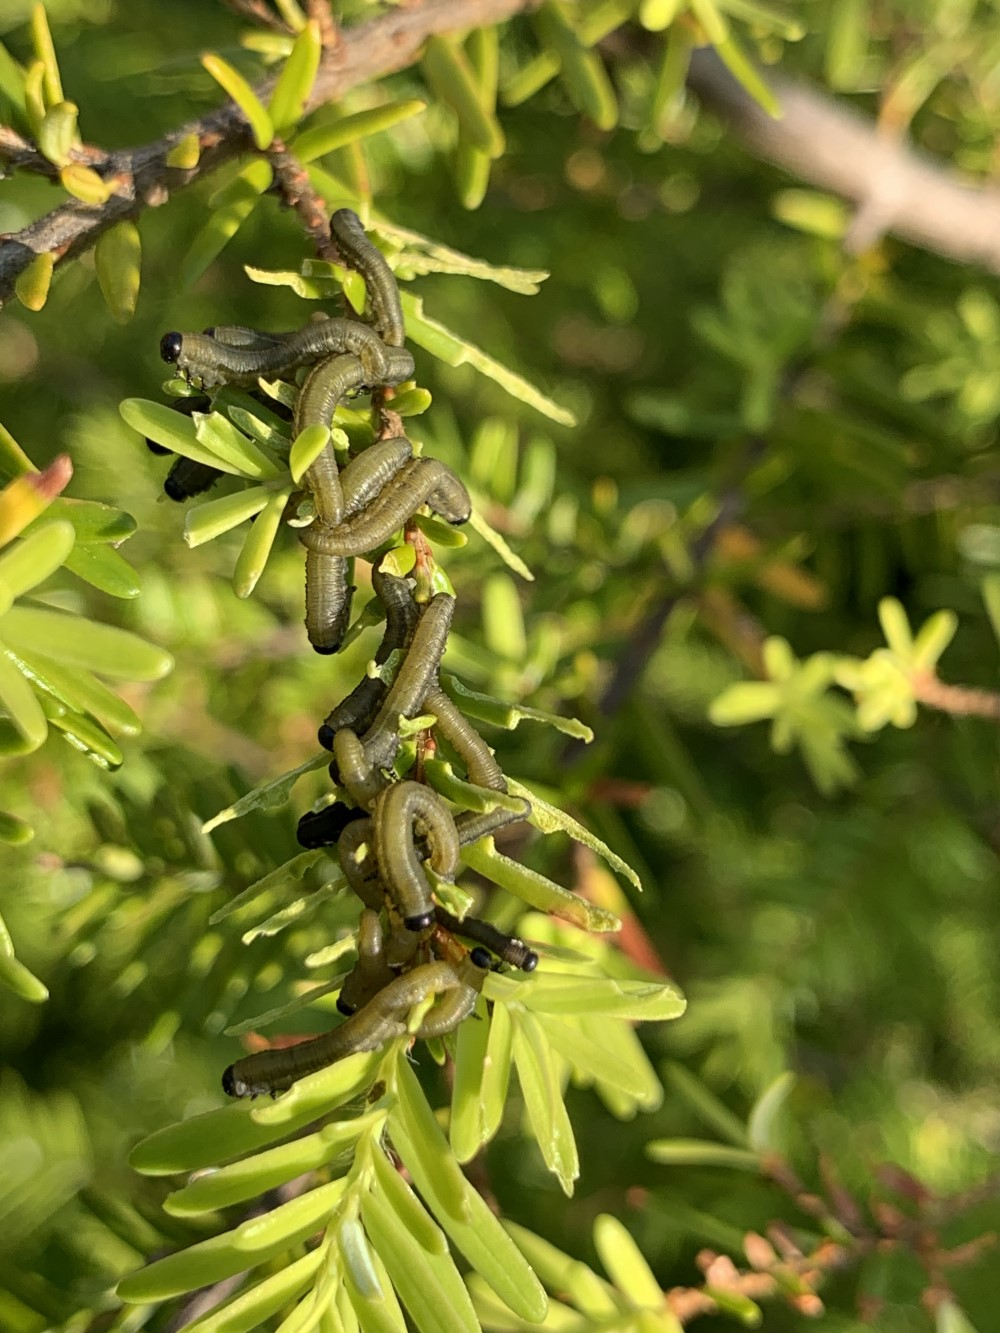
\includegraphics[width=\textwidth]{img/hemlock_sawfly_larvae.jpg}
\caption{Aggregate of hemlock sawfly feeding on western hemlock.}
\label{hemlock_sawfly_larvae}
\end{center}
\end{figure} 

\bibliography{hemlock_sawfly}

